\section{Ótica de dados TbT}

% 2024-05-21-SI_kickedbeam_tbt_acquisitions (tbt-acquisitions)
% 2024-06-11-SI_kickedbeam_tbt_acquisitions (tbt-acquisitions)


\begin{frame}{Ótica de dados TbT: Testes com pingers}

{\footnotesize
\begin{itemize}
    \item estudo dia 2024-05-21 \href{https://ais-eng-srv-ta.cnpem.br/Olog/index.html\#22749\_1}{\beamergotobutton{Olog \#22749\_1}}
    \item scan de delays dos pingers e testes de aquisição TbT
    \item amplitudes menores do que esperadas no feixe quando kickado pelos pingers
    \item desconfiando da temporização, fizemos scan dos \texttt{delay\_raw} para pingh e pingv
    \item delays ótimos encontrados, problema de amplitudes permaneceu
    \item realizamos aquisições varrendo kicks para levantar uma tabela de calibração 
    \item fator de calibração p/ (pingh, pingv) = (1.5417, 1.0227)
\end{itemize} 
}
\begin{figure}
    \centering
    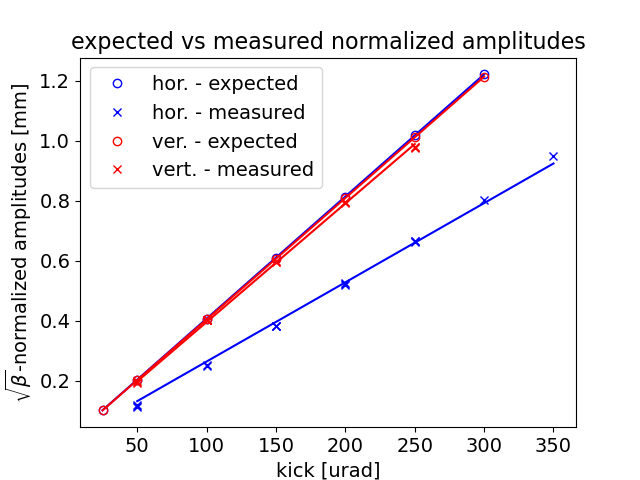
\includegraphics[scale=0.35]{2024-06-21/figures/norm_amp_expected_vs_observed-210524.png}
\end{figure}
\end{frame}



\begin{frame}{Ótica de dados TbT: Medidas de tune-shifts com amplitude}
\begin{minipage}{0.38\textwidth}
    {\footnotesize
    \begin{itemize}
        \item estudo dia 2024-06-11 \href{https://ais-eng-srv-ta.cnpem.br/Olog/index.html\#22749\_1}{\beamergotobutton{Olog \#22749\_1}}
        \item com pingers calibrados, realizamos aquisições TbT do feixe kickado
        \item tunes via espectro dos modos $U$ do SVD da matriz história de $N$ voltas nos 160 BPMs $$X = U \Sigma V^\intercal,  X = [[x_{ij}], [y_{ij}]] \in \mathbb{R}^{N\times 320}$$
    \end{itemize}
}    
\end{minipage}
\hfill
\begin{minipage}{0.58\textwidth}
    \centering
    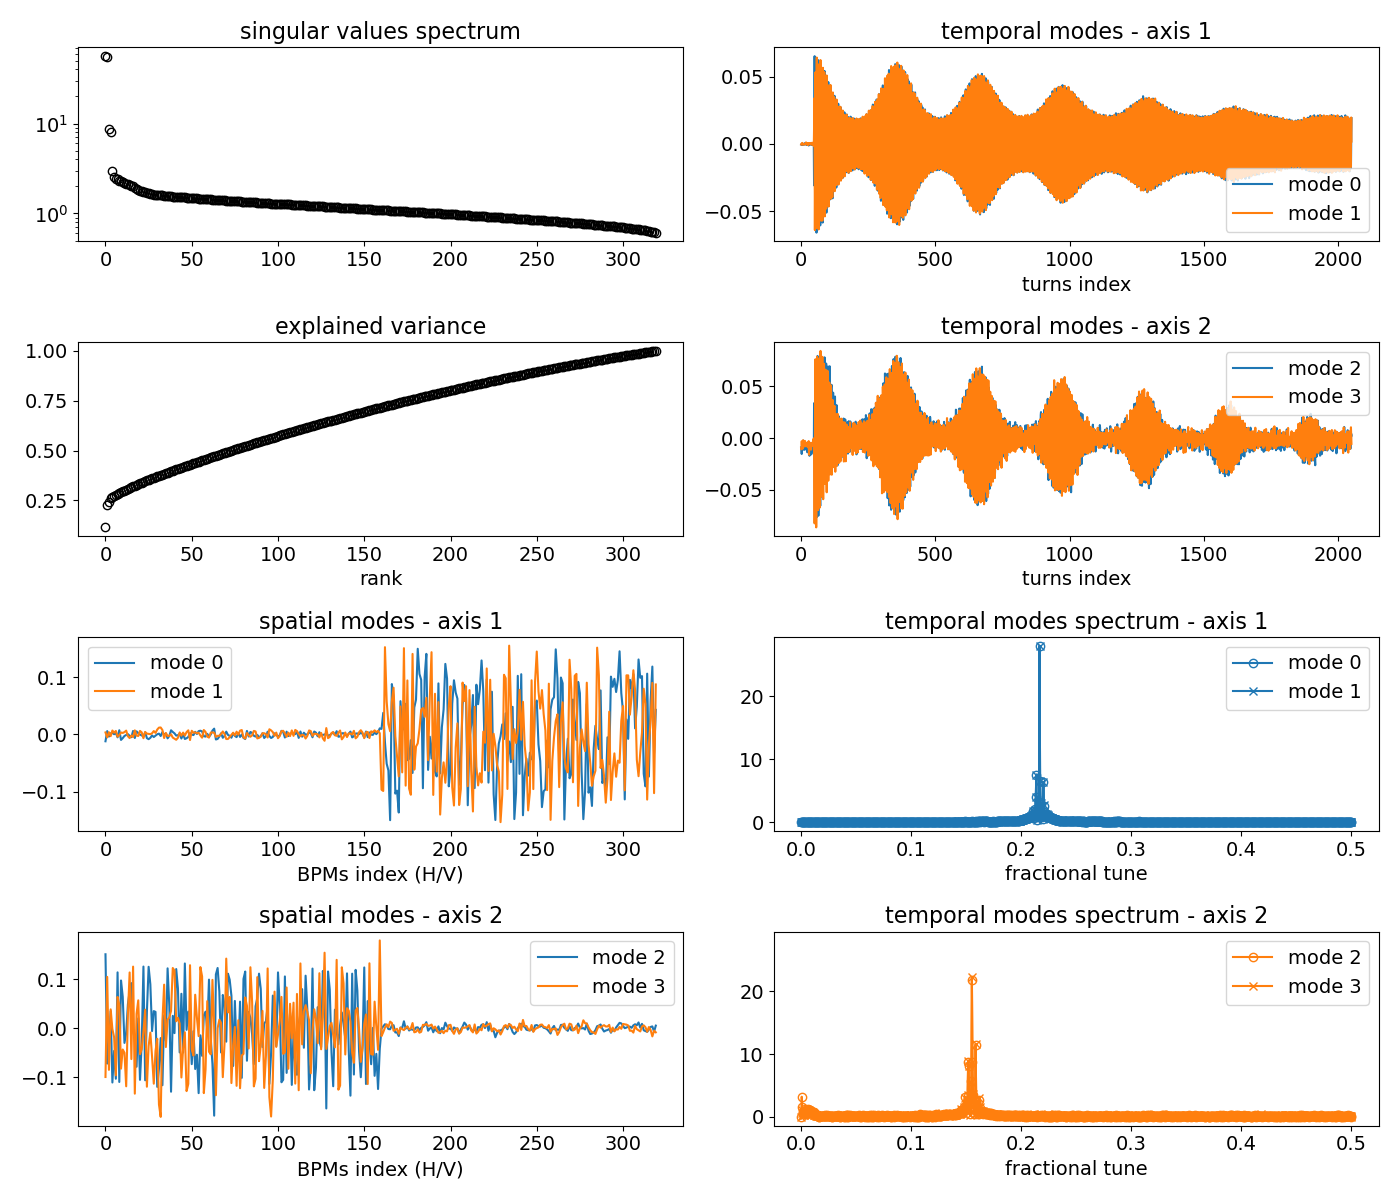
\includegraphics[width=\textwidth]{2024-06-21/figures/tbt_modal_analysis.png}
\end{minipage}
\end{frame}


\begin{frame}{Ótica de dados TbT: Tune-shifts, medidas vs. modelo}

{\footnotesize
\begin{itemize}
    \item regime de tune-shift com amplitude linear (kicks pequenos)
    \item como já esperado, nosso modelo da dinâmica não linear dnão descreve bem a máquina, após a otimização RCDS para novas sintonias.
\end{itemize}
}
\begin{figure}
    \centering
    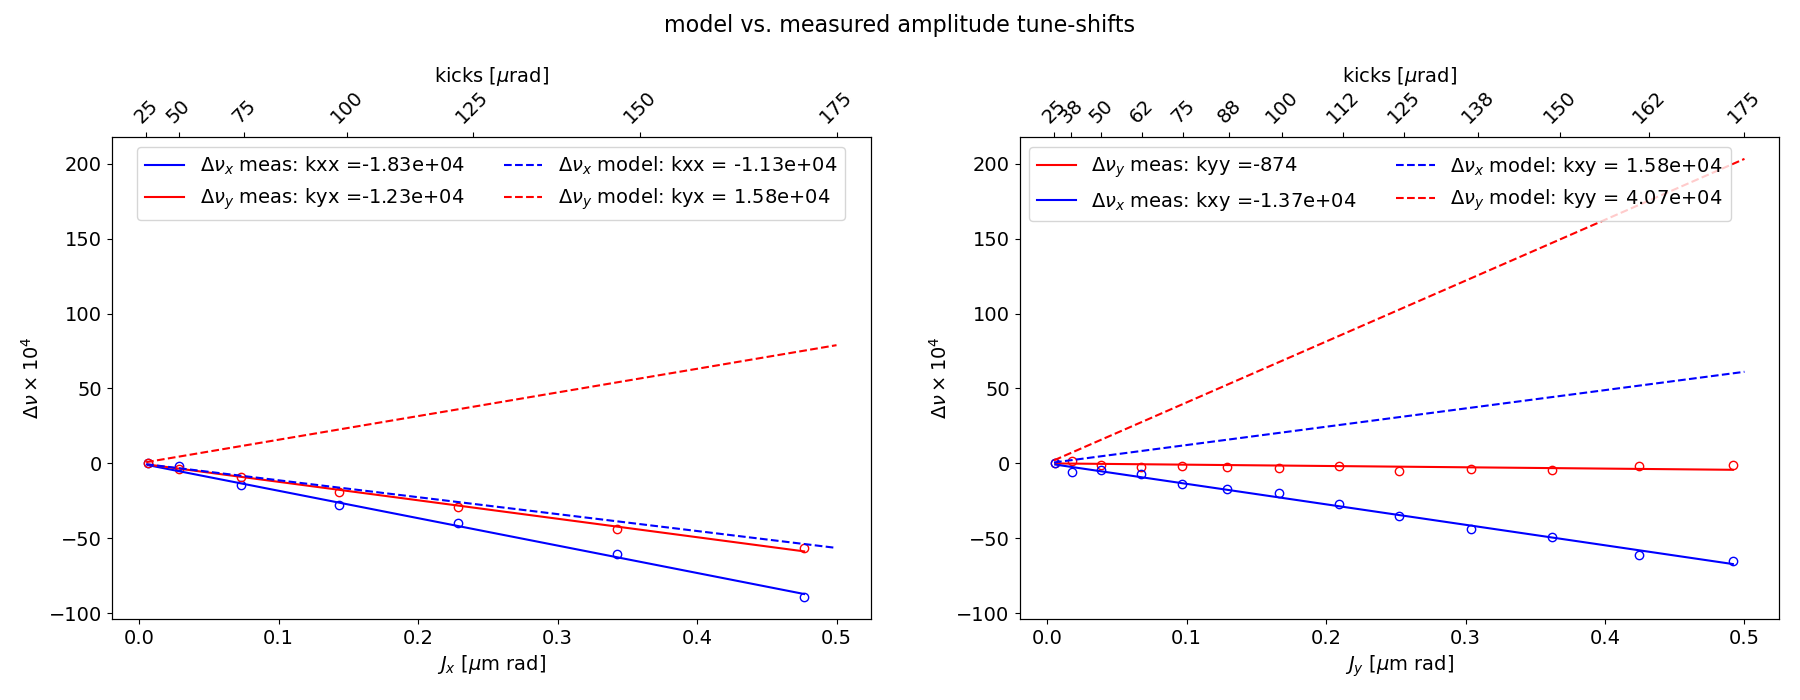
\includegraphics[scale=0.3]{2024-07-12/figures/model_vs_meas_adts.png}
\end{figure}

\end{frame}